\documentclass[tikz,border=8pt]{standalone}
\usetikzlibrary{arrows.meta,positioning}
\begin{document}
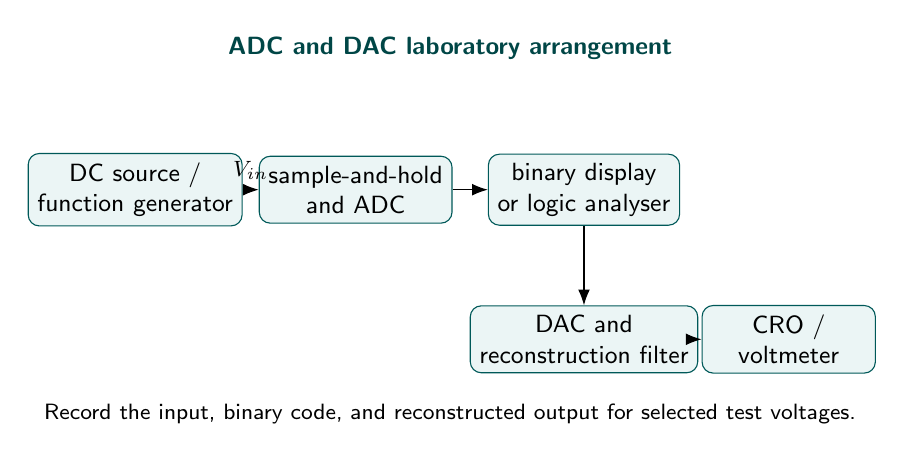
\begin{tikzpicture}[font=\sffamily\small,box/.style={draw=teal!70!black,fill=teal!8,rounded corners,minimum width=2.2cm,minimum height=.85cm,align=center}]
\node[font=\sffamily\bfseries\small,text=teal!55!black] at (0,2.9) {ADC and DAC laboratory arrangement};
\node[box] (source) at (-4,1.1) {DC source /\\function generator};
\node[box] (adc) at (-1.2,1.1) {sample-and-hold\\and ADC};
\node[box] (code) at (1.7,1.1) {binary display\\or logic analyser};
\node[box] (dac) at (1.7,-.8) {DAC and\\reconstruction filter};
\node[box] (scope) at (4.3,-.8) {CRO /\\voltmeter};
\draw[-{Latex[length=2mm]}] (source)--node[above,font=\sffamily\footnotesize]{$V_{in}$} (adc);
\draw[-{Latex[length=2mm]}] (adc)--(code);
\draw[-{Latex[length=2mm]}] (code)--(dac);
\draw[-{Latex[length=2mm]}] (dac)--(scope);
\node[font=\sffamily\footnotesize] at (0,-1.75) {Record the input, binary code, and reconstructed output for selected test voltages.};
\end{tikzpicture}
\end{document}
